\chapter{Results and Analysis}
\label{ch:resultsandanalysis}

This chapter presents the results of both the quantitative and qualitative analysis conducted to evaluate the impact of the Mixed Reality (MR) simulation on participants empathy and emotional responses toward individuals with schizophrenia. It begins with a breakdown of pre-evaluation findings that show baseline attitudes and empathy. Post-evaluation results are then presented, including changes in empathy and emotional states across all participants, as well as specific groups (observer group participants and individual headset users, the experiencers). Statistical comparisons are used to assess whether observed differences are significant. Finally, we integrate observational and verbal feedback from participants to complement the quantitative data. This mixed-methods approach allows for a broader understanding of the simulationss effects.

\section{Demographics}
The study involved n = 29 participants, all of whom are psychology students at the HEdS-FR. Neither age nor gender is asked in the questionnaire, as the focus is on empathy and emotional responses rather than demographic factors and to ensure anonymity. Important to note is all participants in the experiencer group did not have any previous experience with any kind of immersive technology.

\section{Pre-Evaluation Results}
The pre-evaluation phase was conducted prior to any exposure to the simulation. It served to assess baseline levels of empathy and emotional responses towards individuals with schizophrenia. We also gathered information about participants experience with patients, including patients with schizophrenia, as this may affect their perceptions.

\subsection{Experience with Patients and Schizophrenia}

Participants were also asked about their prior experience working with patients in general and specifically with individuals diagnosed with schizophrenia. Responses are recorded on a 5-point scale ranging from 1 (No) to 5 (Yes).

\begin{figure}[H]
    \centering
    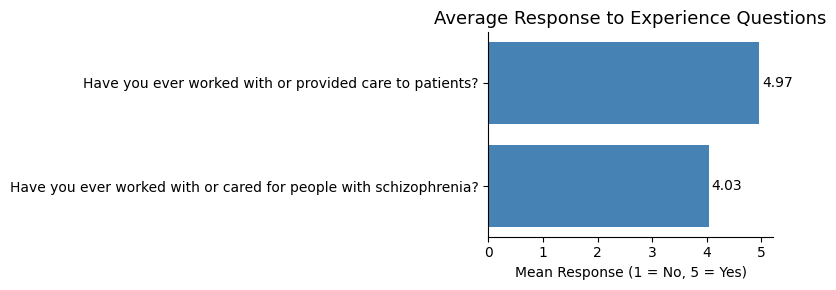
\includegraphics[width=0.7\textwidth]{../../Figures/experience-patients.png}
    \caption{Answers to questions about experience with patients and schizophrenia.}
    \label{fig:experience_patients}
\end{figure}

As shown in Figure~\ref{fig:experience_patients}, nearly all participants reported prior experience working with or caring for patients, with an average response of 4.97. However, fewer had direct experience with individuals with schizophrenia, as indicated by a lower mean score of 4.03. This suggests a general familiarity with healthcare and patient care, but not as much exposure specifically to individuals with schizophrenia. This nuance is why a Likert scale was used as it allows participants to express a level of familiarity rather than a simple "yes" or "no."

\subsection{Baseline Perceptions and Empathy}

Participants responded to a set of 13 Likert-scale items evaluating cognitive and affective components based on the JSE \cite{Hojat2002}. These items were scored from 1 (Strongly Disagree) to 7 (Strongly Agree), with reverse scoring applied to negatively phrased statements.

\begin{figure}[htbp]
    \centering
    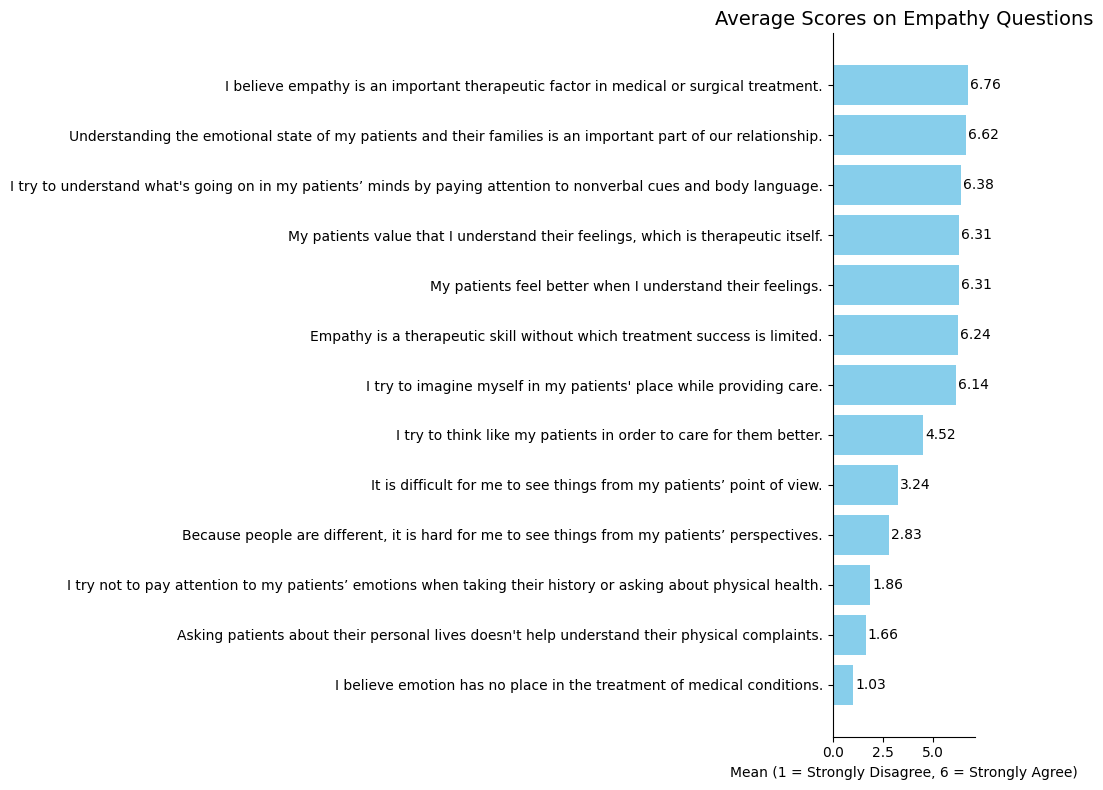
\includegraphics[width=\columnwidth]{../../Figures/avg-scores-pre.png}
    \caption{Average item scores on JSE.}
    \label{fig:avg_scores_pre}
\end{figure}

\vspace{1em}

Figure~\ref{fig:avg_scores_pre} shows the average scores per item. Responses are generally high for positively phrased statements (e.g., “I believe empathy is an important therapeutic factor”), indicating strong baseline attitudes in favor of empathic engagement. In contrast, negatively phrased items (e.g., “I believe emotion has no place in the treatment of medical conditions”) received low agreement, as expected after reverse scoring.

\vspace{1em}

To explore potential variation across groups, empathy scores are also averaged by the time at which participants completed the evaluation session. These groups are constructed based on session start times.

\begin{figure}[H]
    \centering
    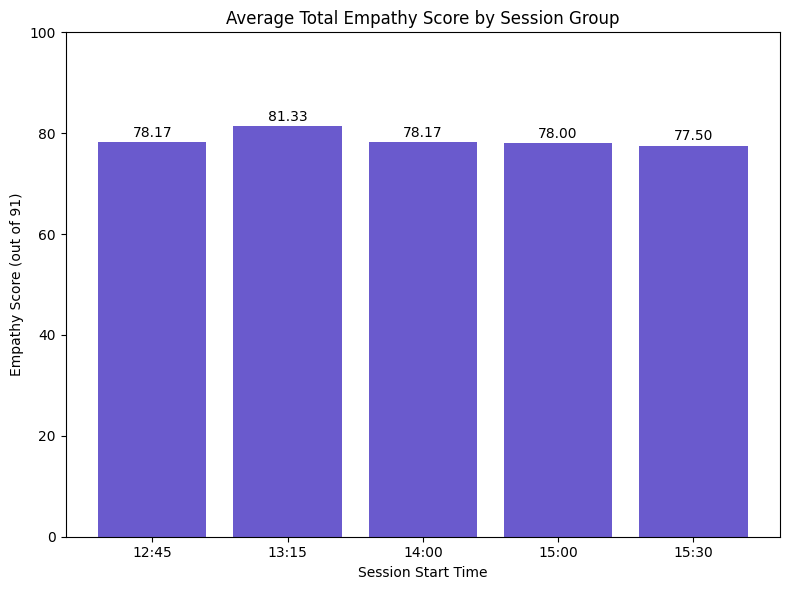
\includegraphics[width=0.75\columnwidth]{../../Figures/avg score-by-group-pre.png}
    \caption{Average total JSE score by group.}
    \label{fig:group_scores_pre}
\end{figure}

As shown in Figure~\ref{fig:group_scores_pre}, total empathy scores are relatively consistent across session groups. The highest group average (81.33) can be observed for the second group, though variation across all of them remained modest (range: 77.50–81.33). The overall mean empathy score across groups is M = 78.63, SD = 1.53, suggesting that time-of-day or group assignment had minimal to no influence on baseline empathy levels.

\begin{figure}[htbp]
    \centering
    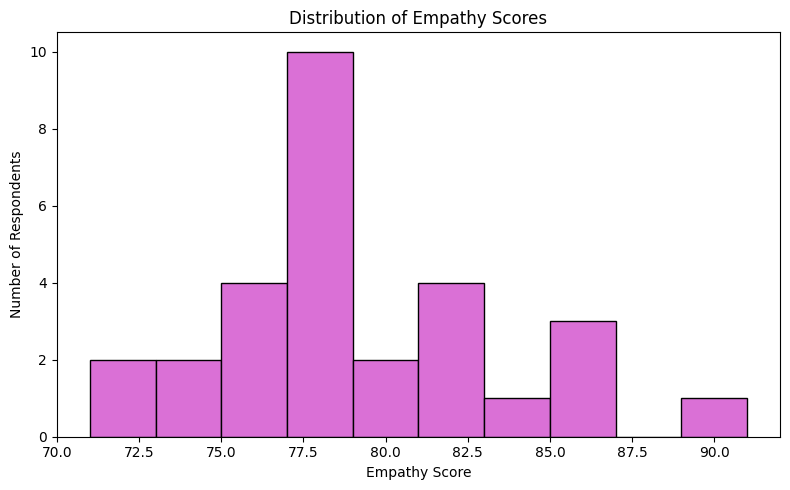
\includegraphics[width=0.75\textwidth]{../../Figures/avg-scores-summary-pre.png}
    \caption{Distribution of total empathy scores among participants.}
    \label{fig:score_distribution_pre}
\end{figure}

\vspace{1em}

Figure~\ref{fig:score_distribution_pre} shows the distribution of total empathy scores. The majority of participants scored between 75 and 85 out of a maximum of 91, which confirms the high initial level of empathy among all students. 

\vspace{1em}

Participants also rated how strongly they associated various emotions with thinking about individuals with schizophrenia, on a scale from 1 (Not at all) to 5 (Extremely).

\begin{figure}[htbp]
    \centering
    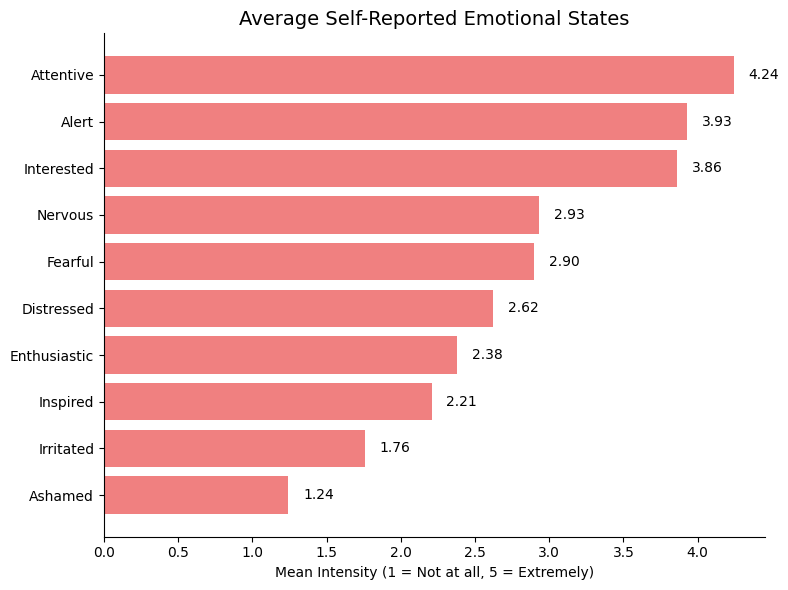
\includegraphics[width=0.7\columnwidth]{../../Figures/avg-emotions-pre.png}
    \caption{Average self-reported emotional intensity associated with thinking about people with schizophrenia.}
    \label{fig:avg_emotions_pre}
\end{figure}

Figure~\ref{fig:avg_emotions_pre} presents the average self-reported intensities for each emotion chosen from the B-PANAS \cite{Boiroux2024}. “Attentive,” “Alert,” and “Interested” ranked highest. This indicates cognitive engagement from the participants. Negative emotions such as “Ashamed” and “Irritated” are reported with lower intensity, which suggests that participants did not associate strong negative feelings with schizophrenia. 

\vspace{1em}

We can already see that pre-evaluation results suggest that participants already showed high levels of empathy. 

\section{Post-Evaluation Results}

Following participation in the experiment, participants (depending on which group (oberserver or experiencer) they were participating in) completed a post-evaluation survey that assessed both empathy levels and emotional states, which features the same question set as the pre-evaluation. These include the JSE \cite{Hojat2002}, and the Brief Positive and Negative Affect Schedule (B-PANAS) \cite{Boiroux2024} to measure emotional responses and perceptions toward individuals with schizophrenia. This section presents the results for all participants divided in two subgroups: those who participated in the group setting, which were observing, and those who experienced the MR simulation individually.

\vspace{1em}

\begin{figure}[H]
\centering
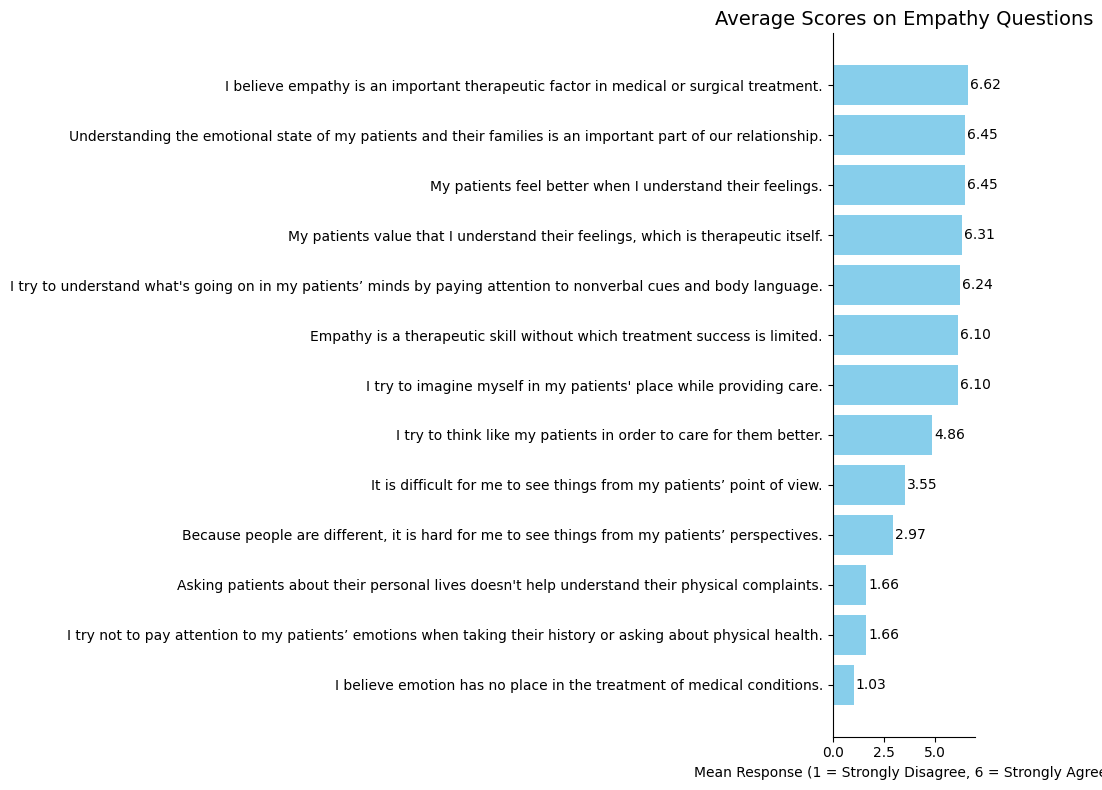
\includegraphics[width=\columnwidth]{../../Figures/avg_scores_post_all.png}
\caption{Average scores on JSE items (After experiment, all participants).}
\label{fig:avg_scores_post_all}
\end{figure}

 The response to the individual JSE items is shown in Figure \ref{fig:avg_scores_post_all}. There is a slight decrease in the average scores for most items compared to the pre-evaluation, but the overall trend remains positive. 

\vspace{1em}

The distribution of empathy scores across all participants is displayed in the Figure \ref{fig:empathy_scores_post_all}. The majority of participants scored high on empathy, with most scores between 75 and 85. The overall mean is M = 78.28, SD= 7.07. This suggests that participants generally maintained a strong sense of empathy after the experiment. However, there are some outliers with lower scores, ranging from 55 to 65, which is interesting, since in the pre-evaluation no one scored this low. This is also indicitated by the high standard deviation. This indicates that while the experiment is effective in maintaining empathy levels for most, a few individuals may have had less engagement or different emotional responses.

\begin{figure}[H]
\centering
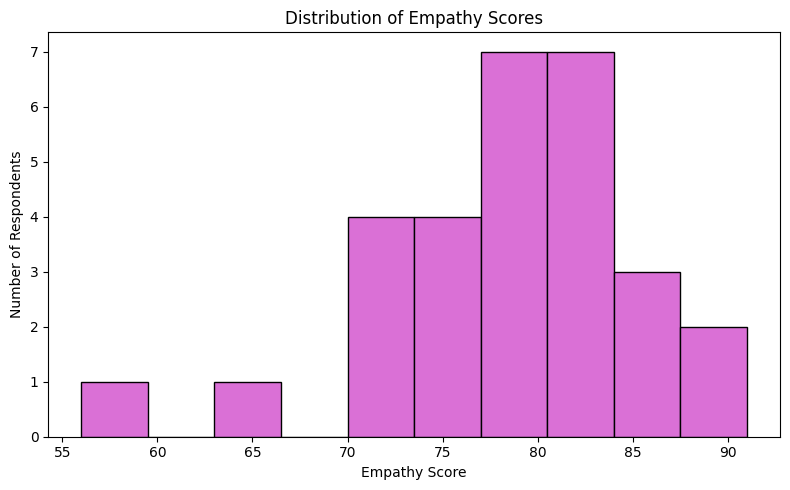
\includegraphics[width=0.75\textwidth]{../../Figures/empathy_scores_post_all.png}
\caption{Distribution of Empathy Scores (After experiment, all participants).}
\label{fig:empathy_scores_post_all}
\end{figure}

\vspace{1em}

The responses to the B-PANAS scale are also asked immediately after the experiment ran through. As shown in Figure~\ref{fig:emotional_post_all}, the responses do not differ a lot from the pre-evaluation results. 

\begin{figure}[htbp]
    \centering
    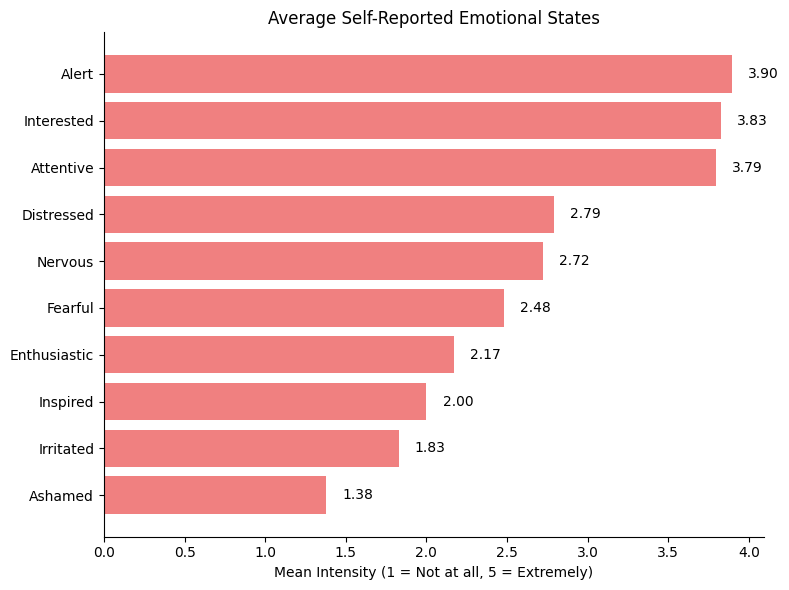
\includegraphics[width=0.75\textwidth]{../../Figures/emotional-post-all.png}
    \caption{Average self-reported emotional states (After experiment, all participants).}
    \label{fig:emotional_post_all}
\end{figure}

A more detailed comparison of pre- and post-scores across the two subgroups will follow in section \ref{sec:pre_post_comparison}.

\subsection{Observer Group Participants}

Participants who took part in the experiment in a group setting (without MR headset) reported emotional responses that are broadly similar to the overall sample. However, their average emotional intensity is slightly higher on items related to cognitive involvement.

\begin{figure}[htbp]
    \centering
    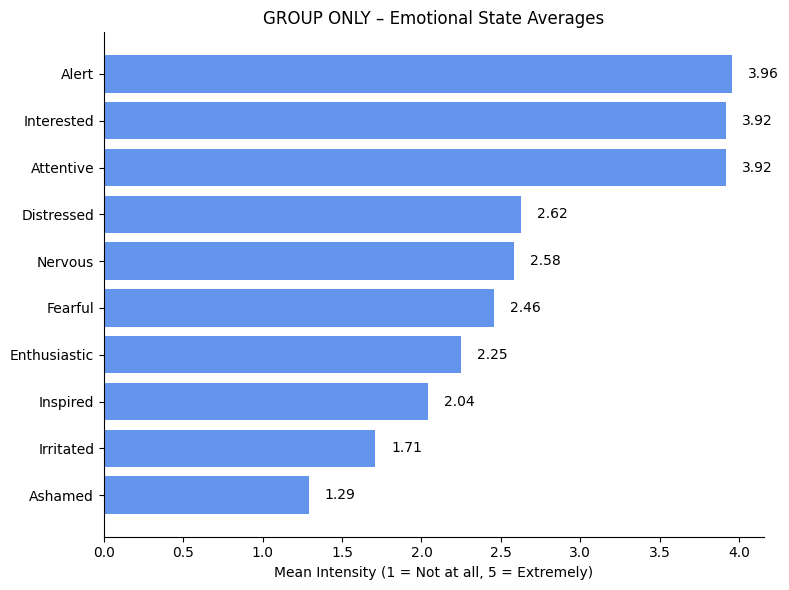
\includegraphics[width=0.75\textwidth]{../../Figures/emotional-post-grp.png}
    \caption{Average emotional state ratings (Oberserver Group only).}
    \label{fig:emotional_post_group}
\end{figure}

As shown in Figure~\ref{fig:emotional_post_group}, \textit{Alert}, \textit{Interested}, and \textit{Attentive} again appeared most strongly. The spread of emotional intensities is relatively consistent with the full group.

\vspace{1em}

The distribution of their overall empathy scores is presented in Figure \ref{fig:empathy_group_post}. The majority of participants in the oberserver group condition scored between 75 and 85 on the empathy scale, but we see again these outliers on the lower end from 55 to 65. The mean is M = 77.79, SD = 7.27 It indicates that while the experiment is effective in maintaining empathy levels for most, again, a few individuals may have had less engagement or different emotional responses. 


\begin{figure}[htbp]
    \centering
    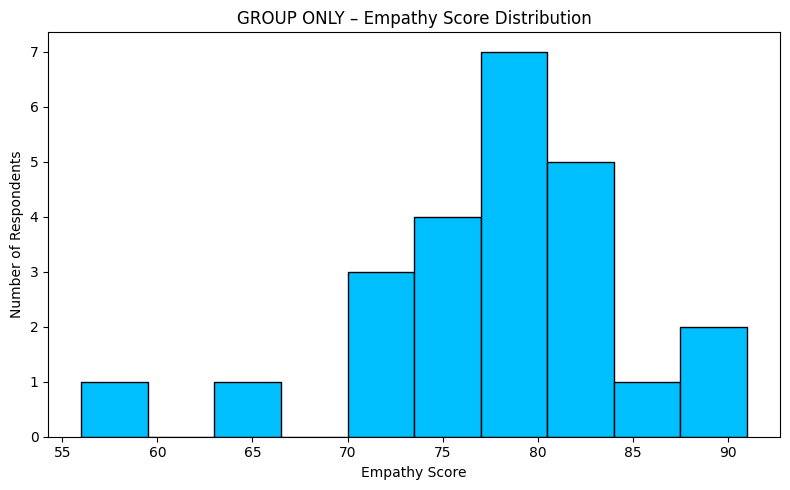
\includegraphics[width=0.75\textwidth]{../../Figures/empathy-score-post-grp.png}
    \caption{Empathy score distribution (Group only).}
    \label{fig:empathy_group_post}
\end{figure}

\vspace{1em}

Session-wise variation in post-experiment empathy scores is shown in Figure~\ref{fig:empathy_group_sessions}. Average scores are relatively stable across session times, ranging from 76.67 to 79.80. The overall mean is M = 78.33, SD = 1.26, the mean being a bit lower than in the pre-evaluation but also the standard deviation is a bit lower. 

\begin{figure}[htbp]
    \centering
    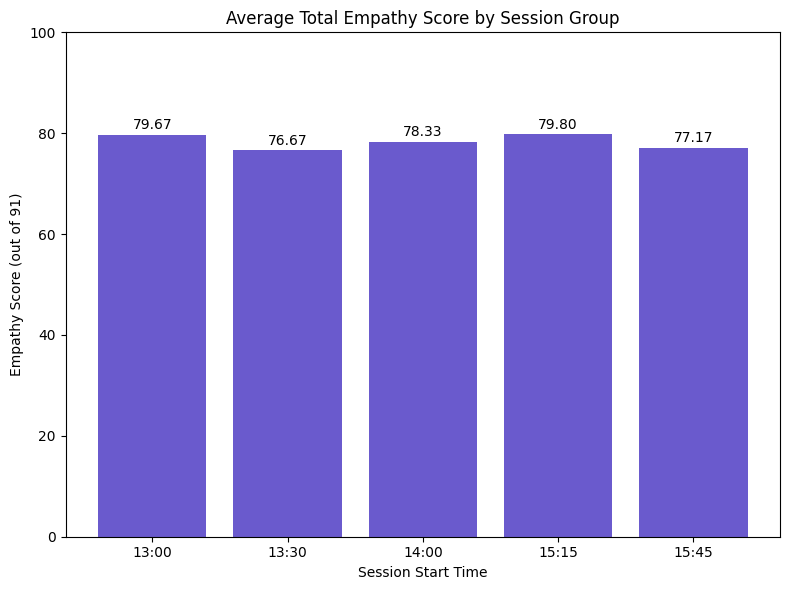
\includegraphics[width=0.75\textwidth]{../../Figures/post-session-grp-empathy.png}
    \caption{Average total empathy score by session time (Group only).}
    \label{fig:empathy_group_sessions}
\end{figure}


\subsection{Experiencer Participants}

Participants who engaged with the MR simulation individually using the headset demonstrated slightly different patterns.As shown in Figure \ref{fig:emotional_post_indiv} their emotional responses included relatively higher levels of \textit{Distress} and \textit{Nervousness}, suggesting a deeper affective impact.

\begin{figure}[H]
    \centering
    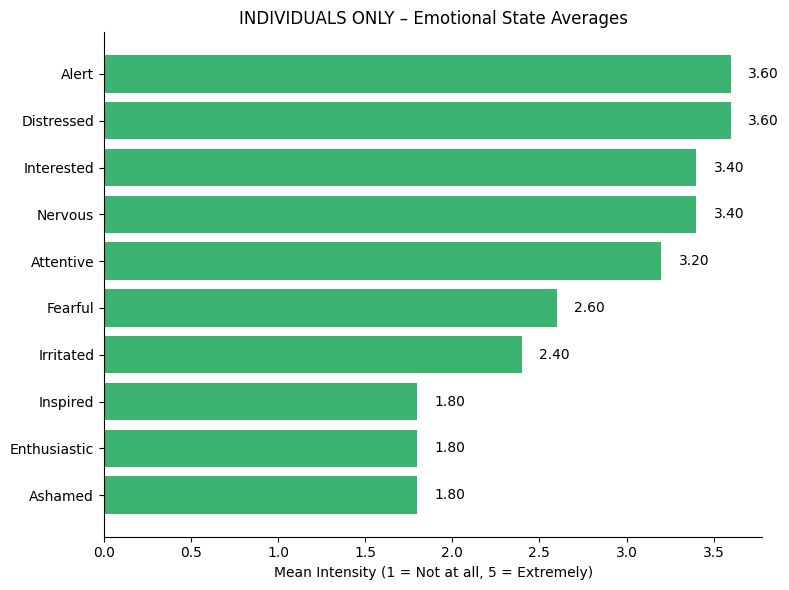
\includegraphics[width=0.75\textwidth]{../../Figures/emotional-post-indiv.png}
    \caption{Average emotional state ratings (Individuals only).}
    \label{fig:emotional_post_indiv}
\end{figure}

Emotions like \textit{Alert} and \textit{Interested} remained high, but they also showed increased ratings for affective states like \textit{Distressed}, \textit{Fearful}, and \textit{Nervous}, suggesting that the immersive simulation may have elicited stronger emotional reactions.

\begin{figure}[htbp]
    \centering
    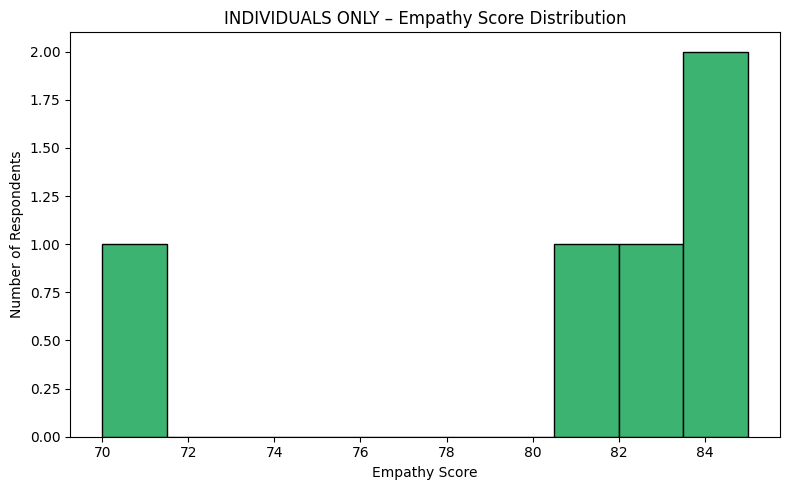
\includegraphics[width=0.75\textwidth]{../../Figures/empathy-score-post-indiv.png}
    \caption{Empathy score distribution (Individuals only).}
    \label{fig:empathy_indiv_post}
\end{figure}

\vspace{1em}

Empathy scores shown in Figure \ref{fig:empathy_indiv_post} in this experiencer group are tightly clustered at the higher end of the scale, indicating that most headset users reported strong empathic attitudes following the simulation. The mean in this evaluation is M = 80.6, SD = 6.1, indicating that the simulation is effective in maintaining empathy levels for most participants, with only a few scoring at around 70.

\subsection{Simulation Evaluation Statements}

Participants were also asked to rate their agreement with various statements evaluating the simulation experience. These were scored on a 7-point scale (1 = Strongly Disagree, 7 = Strongly Agree).

\begin{figure}[H]
    \centering
    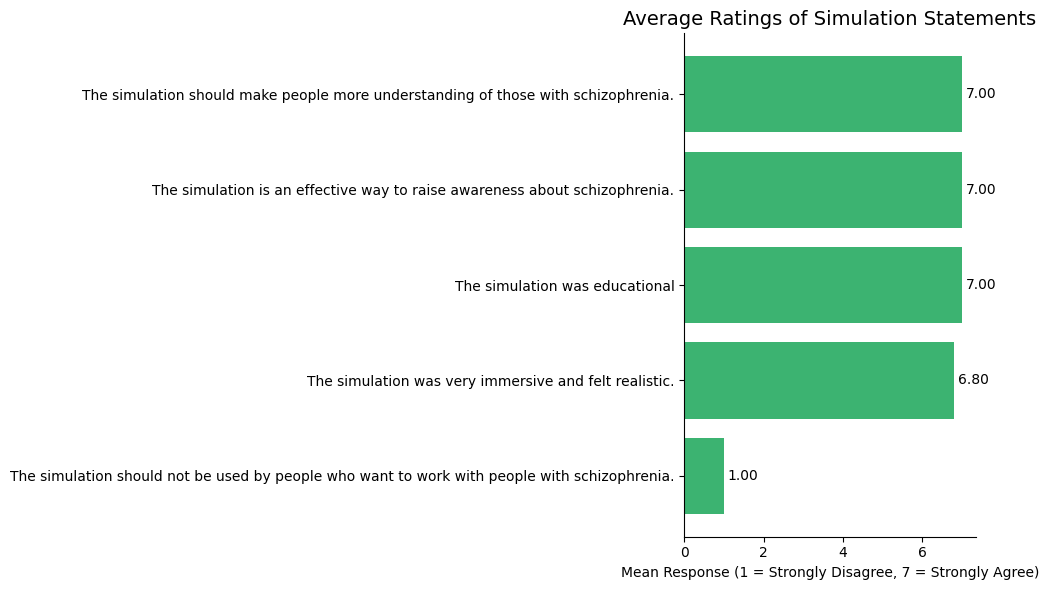
\includegraphics[width=0.9\textwidth]{../../Figures/simulation-evaluation-post.png}
    \caption{Average participant ratings of simulation statements.}
    \label{fig:simulation_evaluation_post}
\end{figure}

Figure~\ref{fig:simulation_evaluation_post} shows that all participants agree on the simulation's educational value, how real it feels, and its ability to increase understanding. The only statement that received strong disagreement is that the simulation “should not be used by people who want to work with people with schizophrenia,” which is a negative statement that is reverse scored. This indicates that participants generally found the simulation to be a valuable educational tool, and they did not believe it should be avoided by future mental health professionals.

\section{Pre vs. Post Comparison Analysis}
\label{sec:pre_post_comparison}
This section presents a statistical comparison of participants empathy and emotional responses before and after the experiment. The analysis features the evaluation whether the experiment led to significant changes in perspective or empathy. Empathy scores, cognitive and affective, and emotion ratings are analyzed using methods suited for this kind of data.

\subsection{Statistical Methods and Hypotheses}

Empathy scores are calculated based on 13 Likert-style items, some of which are reverse-scored. Each participants total empathy score is the sum of their responses. To evaluate changes in emotional response and empathy after the experiment, there is the need to compare pre- and post-evaluation data statistically. The same group of participants completed the questionnaire both before and after the experiment. However, since individual identifiers are not used, it is not possible to link each persons pre- and post-scores directly.

Although the data technically comes from the same group, the lack of matching between responses means that statistical tests designed for paired data (like the paired \textit{t}-test) could not be used. As a result, the pre- and post-evaluazion scores are treated as if they came from two independent groups and an \textbf{independent samples \textit{t}-test} is used instead \cite{independentTtest}.

\paragraph{Hypotheses.} This test compares the average scores from two separate groups and checks whether any difference between them is statistically significant and not random. The hypotheses for the statistical tests are as follows:

\begin{itemize}
  \item \textbf{Null hypothesis ($H_0$):} There is no difference in empathy scores between the pre- and post-evaluation.
  \item \textbf{Alternative hypothesis ($H_1$):} There is a difference in empathy scores between the pre- and post-evaluation.
\end{itemize}


\subsection{Statistical Test Results}

To assess the impact of the experiment, we applied statistical tests to compare pre- and post-evaluation responses with significance evaluated at $p < 0.05$.

\subsubsection{Empathy Score Comparison}

We compared pre- and post-evaluation empathy scores using a independent \textit{t}-test to assess the effect of the experiment.

\begin{table}[htbp]
    \centering
    \caption{Empathy scores (pre- and post-experiment)}
    \begin{tabular}{|l|c|c|c|}
        \hline
        \textbf{Condition} & \textbf{Mean} & \textbf{Standard Deviation} & \textbf{n} \\
        \hline
        Pre-experiment & 78.66 & 4.44 & 29 \\
        \hline
        Post-experiment & 78.28 & 7.07 & 29 \\
        \hline
    \end{tabular}
    \label{tab:group_empathy_stats}
\end{table}

The results from the independent \textit{t}-test are:

\begin{itemize}
    \item \textit{t}-value = \(-0.245\)
    \item \textit{p}-value = \(0.808\)
\end{itemize}

The very small difference between the pre- and post-experiment scores, combined with a high \textit{p}-value, suggests that the experiment did not lead to a statistically significant change in empathy levels. It is worth noting that this result does not necessarily mean the experiment had no effect. The inability to match individual responses may have reduced the sensitivity of the analysis. A future study with identifiable paired responses would allow for a more accurate test of change.

\vspace{1em}

Therefore, it is necessary to accept the null hypothesis and reject the alternative hypotheses. While the mean empathy score decreased slightly from pre to post-evaluation, the difference is not statistically significant. This suggests that the experiment may not have produced a measurable change in empathy, or that individual effects vary too widely to view n overall change.

\paragraph{Visualizations}

To further explore the effect of the experiment on participant empathy, both the distribution of empathy scores and individual-level changes from pre- to post-evaluation are visualized. 

\begin{figure}[htbp]
    \centering
    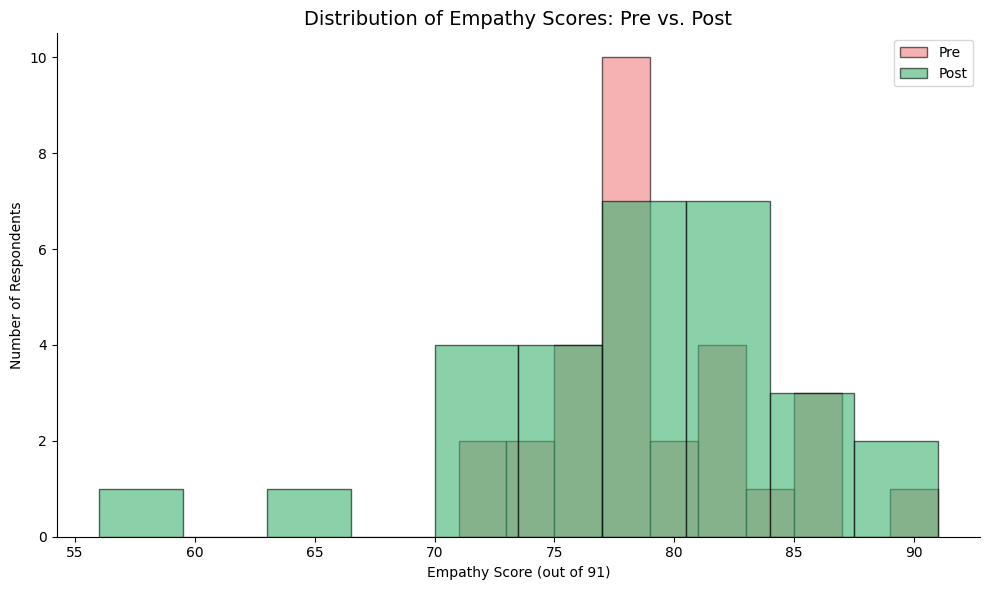
\includegraphics[width=0.75\textwidth]{../../Figures/emp-comparison.png}
    \caption{Distribution of Empathy Scores Before and after the experiment.}
    \label{fig:empathy_dist_hist}
\end{figure}

Figure~\ref{fig:empathy_dist_hist} shows the histogram of empathy scores before and after the experiment. Both sets of scores look quite similar, with most people scoring between 70 and 85. After the experiment, the scores spread out a bit more—some people scored a little lower, but there is also a slight increase at the higher end. This suggests that while some participants may have become more empathic, the overall shape of the distribution did not change much.

\begin{figure}[htbp]
    \centering
    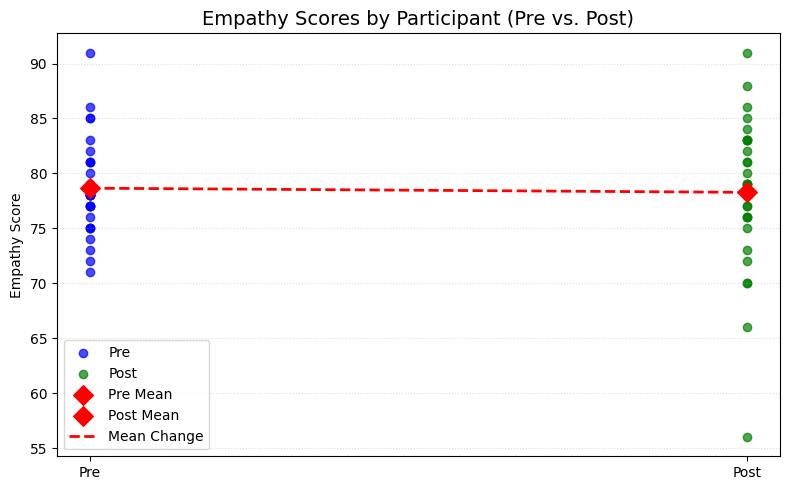
\includegraphics[width=0.75\textwidth]{../../Figures/emph-comparison-means.png}
    \caption{Empathy Scores by Participant: Pre vs. Post with Mean Comparison.}
    \label{fig:empathy_means_line}
\end{figure}

\vspace{1em}

In Figure~\ref{fig:empathy_means_line}, each dot represents a participants empathy score before and after the experiment. Red diamonds indicate the group means, and the dashed red line connects the mean pre- and post-scores. This visualization confirms that although the individual scores are distributed across a similar range, the overall mean remained effectively stable. A few participants show noticeable changes in either direction, but the majority maintained consistent empathy scores. The mean dropped slightly from 78.66 (pre) to 78.28 (post), as also reflected in the results of the independent smaples \textit{t}-test ($p = 0.808$). This supports the interpretation that the experiment did not result in a statistically significant change in overall empathy levels.

\paragraph{Comparison by Group}

These graphs underscore the importance of looking beyond averages: while the overall effect is minimal, some individuals experienced increases or decreases that could be explored further—especially through qualitative methods or subgroup analysis. To examine potential group-level effects, average empathy scores are compared across different session groups. This comparison is based on observations made during the experiment sessions: in some groups, the participant wearing the headset responded with visible engagement, like verbal comments, physical reactions, or other expressions. In others, the headset user appeared more passive. Since the experiment is designed to promote empathy through a shared experience, this variation in participant engagement is considered a possible factor influencing group-level outcomes.


\begin{figure}[htbp]
    \centering
    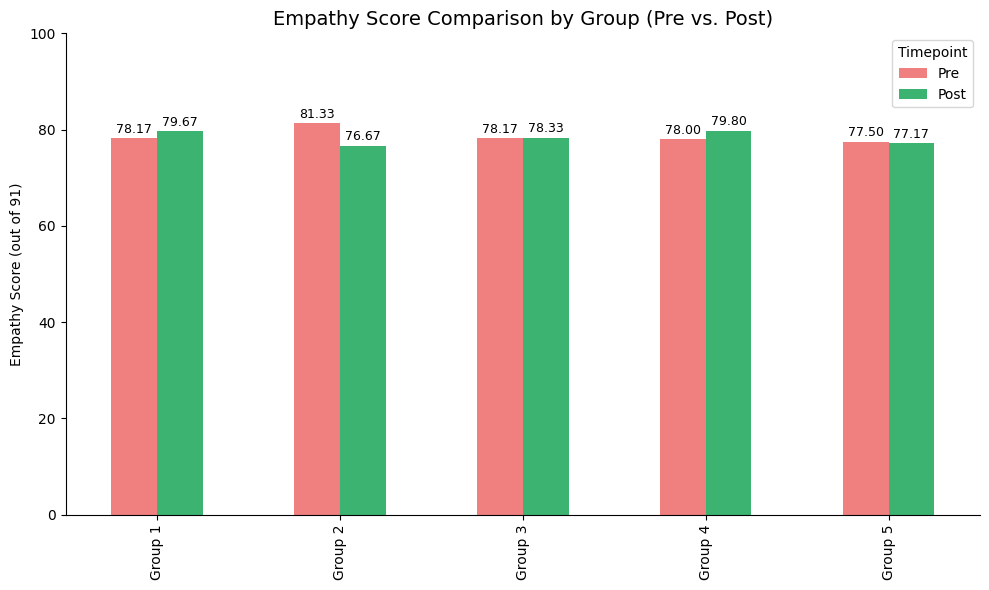
\includegraphics[width=0.85\textwidth]{../../Figures/emph-scores-comp-grp.png}
    \caption{Empathy Score Comparison by Group (Pre vs. Post).}
    \label{fig:empathy_group_bar}
\end{figure}

\vspace{1em}

Figure~\ref{fig:empathy_group_bar} illustrates mean empathy scores for each group before and after the experiment. The scores remain stable across all groups, with small increases observed in Groups 1, 3, and 4, and small decreases in Groups 2 and 5. None of these differences are large enough to suggest a meaningful group-specific effect. This reinforces the previous conclusion that the experiment did not produce a systematic shift in overall empathy scores.

\paragraph{Cognitive vs. Affective Empathy}

To better understand the nature of the empathy being measured, the total score is into two subcomponents: \textit{cognitive empathy}, which reflects perspective-taking and understanding mental states; and \textit{affective empathy}, which involves emotional resonance and compassion.

\begin{figure}[htbp]
    \centering
    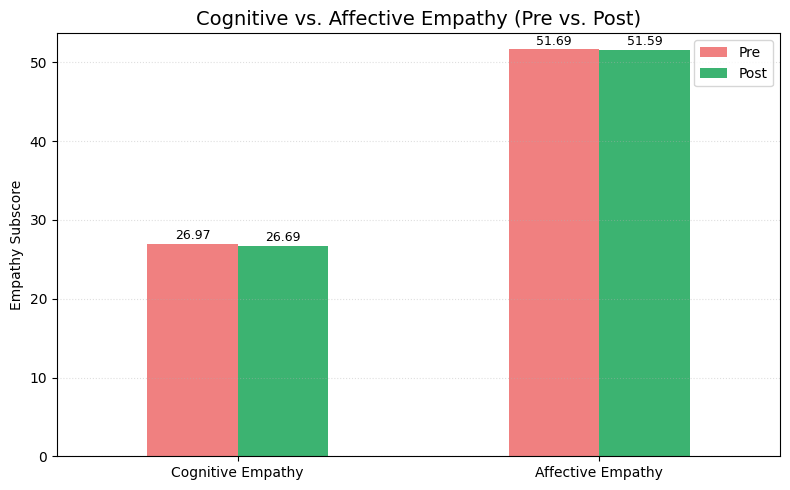
\includegraphics[width=0.75\textwidth]{../../Figures/cog-vs-affect.png}
    \caption{Cognitive vs. Affective Empathy Scores (Pre vs. Post).}
    \label{fig:empathy_cog_aff}
\end{figure}

\vspace{1em}

As shown in Figure~\ref{fig:empathy_cog_aff}, the scores remained nearly the same before and after the experiment. Cognitive empathy dropped slightly from 26.97 to 26.69, and affective empathy also showed a small decrease from 51.69 to 51.59. These minimal changes suggest that the experiment did not have a meaningful impact on either aspect of empathy. This breakdown supports the earlier results, reinforcing the interpretation that the experiment had little effect on participants reported empathy levels immediately after the experience.

% \subsection{Comparison: Individual Headset Users vs. Pre-Evaluation Group}

% To assess whether the most immersive condition—the individual use of the MR headset—was associated with greater empathy, we conducted an exploratory comparison between the post-evaluation scores of headset users ($n=5$) and the pre-evaluation scores of the full participant group ($n=29$).

% The average empathy score for headset users was slightly higher (80.6) than that of the pre-evaluation group (78.7). To test whether this difference was statistically meaningful, we applied the Mann–Whitney U test, a non-parametric method appropriate for comparing two independent groups.

% \begin{itemize}
%   \item \textbf{Mean (Pre-Evaluation Group):} 78.66
%   \item \textbf{Mean (Individual Headset Users):} 80.60
%   \item \textbf{Mann–Whitney U test:} $U = 48.0,\ p = 0.2409$
% \end{itemize}

% As the p-value exceeds the conventional significance threshold of $0.05$, we fail to reject the null hypothesis and conclude that the observed difference is not statistically significant. Nevertheless, the direction of the effect—higher empathy among headset users—may suggest a potential trend.

% \begin{figure}[htbp]
%     \centering
%     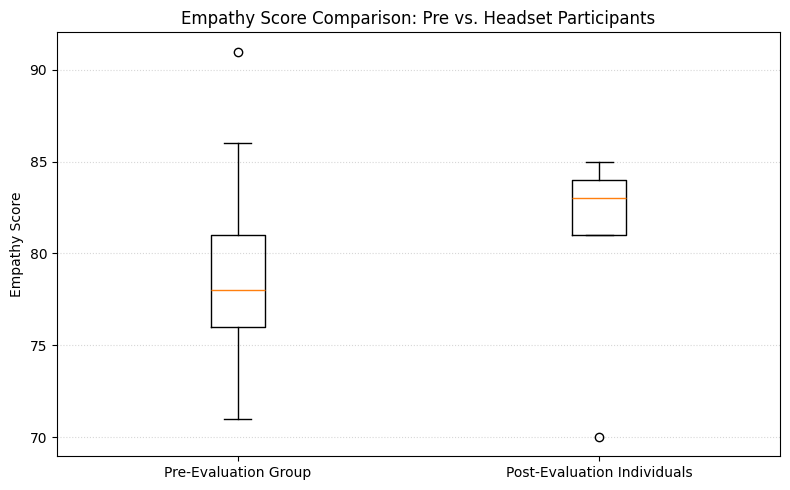
\includegraphics[width=0.75\textwidth]{../../Figures/boxplot-indiv.png} 
%     \caption{Empathy score comparison between individual headset users and pre-evaluation group.}
%     \label{fig:boxplot_indiv_vs_pre}
% \end{figure}

% Given the very small sample size of the individual condition, these results should be interpreted cautiously. However, they offer a potentially meaningful signal: the immersive, embodied experience may have contributed to slightly elevated empathic responses. Future studies should explore this with larger samples and through the integration of qualitative data on individual experiences.


\subsubsection{Emotional Response Comparison}

To explore whether participants emotional responses toward people with schizophrenia changed after the experiment, independent samples \textit{t}-tests are conducted for each of the ten emotion items. Even though the same group completed the survey before and after the experience, the responses could not be linked individually, so the analysis treated them as two separate groups.

\paragraph{Hypotheses.} For each emotion, the following hypotheses are tested:

\begin{itemize}
    \item \textbf{Null Hypothesis ($H_0$):} There is no difference in the average intensity of the emotion between the pre and post-experiment groups.
    \item \textbf{Alternative Hypothesis ($H_1$):} There is a difference in the average emotional intensity between the pre and post-experiment groups.
\end{itemize}


\begin{table}[H]
\centering
\caption{Independent Samples \textit{t}-Test Results for Emotional Changes}
\begin{tabular}{|l|c|c|c|c|c|}
\hline
\textbf{Emotion} & \textbf{Pre Mean} & \textbf{Post Mean} & \textbf{t-statistic} & \textbf{p-value} & \textbf{Significant} \\
\hline
Attentive     & 4.24 & 3.79 & -1.924 & 0.0599 & False \\
Fearful       & 2.90 & 2.48 & -1.287 & 0.2041 & False \\
Ashamed       & 1.24 & 1.38 &  0.800 & 0.4273 & False \\
Enthusiastic  & 2.38 & 2.17 & -0.768 & 0.4458 & False \\
Inspired      & 2.21 & 2.00 & -0.756 & 0.4526 & False \\
Nervous       & 2.93 & 2.72 & -0.603 & 0.5491 & False \\
Distressed    & 2.62 & 2.79 &  0.503 & 0.6176 & False \\
Irritated     & 1.76 & 1.83 &  0.215 & 0.8305 & False \\
Alert         & 3.93 & 3.90 & -0.128 & 0.8983 & False \\
Interested    & 3.86 & 3.83 & -0.113 & 0.9104 & False \\
\hline
\end{tabular}
\label{tab:ttest_emotions}
\end{table}

None of the emotions showed a statistically significant difference between the pre- and post-experiment answers at the $p < 0.05$ level. However, the emotion \textit{Attentive} came close to significance ($p = 0.0599$), suggesting a possible decline in attentiveness after the experiment, though this trend did not reach the set threshold for statistical significance.

\vspace{1em}

To better understand the direction and size of the changes, Figure~\ref{fig:emotion_change} shows the average difference for each emotion (post minus pre). Positive values reflect increased emotional intensity following the experiment, while negative values indicate a decrease.


\begin{figure}[H]
    \centering
    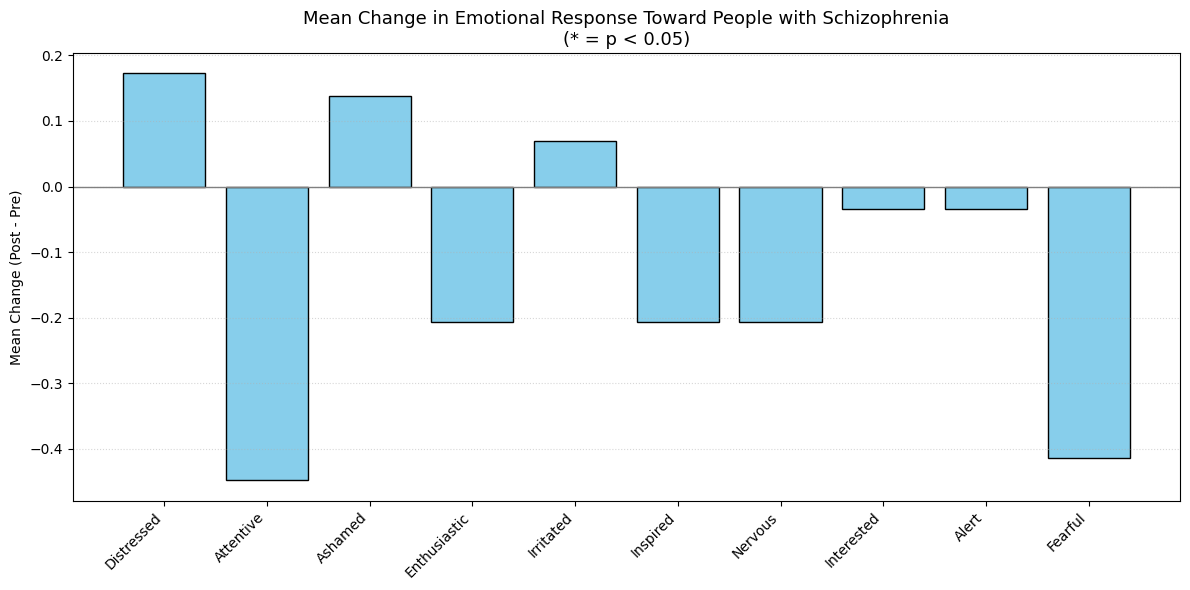
\includegraphics[width=0.85\textwidth]{../../Figures/mean-change-emotions.png}
    \caption{Mean change in emotional response toward individuals with schizophrenia.}
    \label{fig:emotion_change}
\end{figure}

Even though the changes are not statistically significant, the Figure shows some patterns in how the emotions of the participants shifted. For example, there are small increases in emotions like \textit{Distressed}, \textit{Ashamed}, and \textit{Irritated}. At the same time, feelings like \textit{Fearful} and \textit{Nervous} showed slight decreases.

\vspace{1em}

These patterns suggest that the experiment may have influenced how some people felt, but the changes are not strong or consistent enough to be considered meaningful. A larger sample or follow-up interviews might help capture more of these individual emotional reactions.

\section{Mixed Methods Integration}
In addition to statistical analyses, observational and self-reported qualitative data are collected to complement the quantitative findings. This included observations during the MR experience, comments after the experiment, and other feedback where available. Participants who wore the MR headset shared reflections that contextualized their questionnaire responses. These insights helped explain individual variability and added understanding of the experiments emotional impact.


\subsection{Participant Experience and Observational Feedback}

During each session, one participant wore the MR headset simulating auditory and visual hallucinations while attempting to complete a simple task. The rest of the group observed and participated in the same task under normal conditions. This design aimed to allow both the headset user to experience symptoms first-hand and the group to witness their visible effects, ideally having an effect on empathy through both perspectives.

\vspace{1em}

How participants behaved was very varied. Some headset users showed visible signs of discomfort, such as pinching their lips, turning their heads, hesitating, or seeking clarification. Others remained largely focused on the task, displaying minimal reaction to the simulation.

\begin{figure}[H]
    \centering
    
\includegraphics[width=0.85\textwidth]{../../Figures/Group-02-movingArm.jpg}
    \caption{Example of group 2 where participant interacted with the dots.}
    \label{fig:simulation-interaction}
\end{figure}

\vspace{1em}

Oberserver group reactions also varied: in some cases, there were uneasy chuckles, concerned glances, or verbal encouragements (“be brave,” “do you need help?”). In other groups, external participants were mostly unaware of the internal struggle the headset user was experiencing, sometimes even forgetting the headset was even present. An example of a participant interacting with the simulation directly is shown in Figure \ref{fig:simulation-interaction}

\vspace{1em}

Table~\ref{tab:qual_summary} provides a summary of observations made during each experiment session, combining notes on the behavior of the participant using the headset, the reactions from the observers, and direct quotes from participants. This overview helps illustrate how differently each session was, with regards to the emotional response, and group dynamics. The qualitative details offer context for interpreting the experiments impact, especially in cases where verbal or emotional responses were more visible during or after the experience.

\begin{table}[H]
\centering
\caption{Summary of Headset User Experience and Observer Group Reactions}
\begin{tabular}{|c|p{4.2cm}|p{4.2cm}|p{4.8cm}|}
\hline
\textbf{Group} & \textbf{Headset User Behavior} & \textbf{Observer Group Reaction} & \textbf{Key Participant Quotes} \\
\hline
Group 1 & Nervous laughter, looked around, avoided interacting with virtual elements, reported confusion. & Limited group reaction; one participant quietly offered encouragement. & “The voices keep pulling you down.” \newline “It’s persecution.” \newline “I now understand my cousin [who has schizophrenia] better.” \\
\hline
Group 2 & Initially not reactive, later visibly overwhelmed, touched spheres, slight disorientation. & Mild group curiosity, one noted concern, most forgot headset was active. & “There was too much information.” \newline “I forgot the instructions.” \newline “It's harder not to do what the voices say.” \\
\hline
Group 3 & Visibly uncomfortable, delayed task start, repeated lip-pinching, eventually emotional. & Group unaware during task, visibly moved after, discussion emerged post-simulation. & “It was horrible.” \newline “I couldn't concentrate... even now I don't know.” \newline “If 2 minutes is absorbing, I can't imagine the people who feel that way every day.” \\
\hline
Group 4 & Focused externally, but no interaction with visual stimuli. Seemed shocked post-experience. & Participant’s distress was internalized; group noticed little during the task. Two members heard audio leaks. & “The voices were disturbing.” \newline “Living the symptoms is another level of experience.” \newline “I think I have more empathy now.” \\

\hline
Group 5 & Started quickly but showed signs of discomfort; pinched lips and waited impatiently for the end. & Group was mostly unaware of the participant’s inner struggle. & “It took a lot of energy and concentration.” \newline “The longer it took, the more frightening it became.” \newline “The simulation helped me realize what they go through.” \\

\hline
\end{tabular}
\label{tab:qual_summary}
\end{table}

\subsubsection{Verbal Feedback from Participants during Debrief}

Several individuals who experienced the simulation described strong emotional and cognitive impact during the debrief. Themes included difficulty concentrating, feeling overwhelmed, dissonance between task instructions and intrusive voices, and a greater understanding of what people with schizophrenia might endure. Some illustrative quotes include:

\begin{itemize}
  \item “We try to focus on something good but the voices keep pulling you down.”
  \item “At first I really didn't want to listen to the voices, but then I couldn't… It's harder not to do what the voices say.”
  \item “I couldn’t understand the instructions… even now I don’t know what we were supposed to do.”
  \item “It was horrible. The voices made simple tasks feel impossible.”
  \item “It was emotionally sad… I didn’t want to look up because I was scared of what I’d see.”
  \item “It took a lot of concentration… I was glad when it was over.”
  \item “I remember my cousin has schizophrenia… now I feel like I better understand what he feels.”
\end{itemize}

Observers also shared reflections:

\begin{itemize}
  \item “I forgot she was wearing the headset… then I saw her moving strangely and I got worried.”
  \item “Seeing her struggle was emotional. It changed how I think about people with schizophrenia.”
  \item “She didn’t react much, so I didn’t realize it was hard for her.”
\end{itemize}

\subsubsection{Interpretation and Reflection}

The reflections shared during the debrief conversations help explain why the empathy scores did not show strong changes. Even though the numbers stayed mostly the same, many participants described feeling deeply affected by the simulation in ways that are hard to measure with a questionnaire.

One common theme is how overwhelming the auditory hallucinations were. Many participants said the voices were much more distracting than the visual effects or the instructions. Some said they felt confused during the task, distracted by the voices. The overall tone from participants after the experience is that they described seeing things differently afterward, with a stronger sense of empathy or understanding for people living with these symptoms.

\vspace{1em}

Importantly, the visibility of the experience to observers varied greatly. In some groups, the headset users reactions were subtle or absent, making it difficult for others to relate or observe andything interesting at all. In others, discomfort or confusion was clearly visible and provoked reactions among the others. This variation highlights the importance of guided debriefs and shared reflection to fully activate the empathy potential of such simulations.

\vspace{1em}

While the simulation may not have changed self-reported empathy scores, these qualitative accounts suggest that for many participants, the experience was personally impactful. The participants were also in agreement that this setup would make sense as a future education tool, which is promising for future applications in mental health training.


\section{Summary of Key Findings}

The results of this mixed-methods study suggest that while the experiment did not produce statistically significant changes in empathy scores across the entire sample, it nevertheless produced meaningful cognitive and emotional engagement for many participants. Pre-evaluation results indicated that students began the experiment with relatively high levels of empathy and attentiveness, leaving limited room for  movement in quantitative scores. This is particularly evident in the JSE, where most participants scored in the upper range both before and after the experiment.

\vspace{1em}

Post-evaluation data confirmed that self-reported empathy remained largely stable. Neither the total empathy scores nor the scores of cognitive and affective empathy showed significant change following the experiment, and statistical comparisons did not support the alternative hypothesis. Similarly, emotional affect scores from the B-PANAS showed only modest variation pre- and post-evaluation, with none reaching statistical significance. Despite these findings, certain trends were observed, such as a modest decrease in attentiveness and also increases in distress-related emotions for headset users.

\vspace{1em}

The qualitative findings are more revealing, which offered insight into participants experiences. Headset users frequently described strong emotional reactions to the simulation, including difficulty focusing, feelings of helplessness and emotional discomfort. Many noted that the experience altered how they viewed people living with schizophrenia, leading to greater compassion and understanding. Observers also reported increased awareness, particularly when they noticed visible signs of struggle in the headset user.

The experiment was broadly perceived as educational and realistic, with participants agreeing that it helped raise awareness about schizophrenia and could be valuable for those preparing to work in mental health care. These reflections helped surface emotional and empathetic responses that are not always visible in the questionnaires but nevertheless shaped their learning.

\vspace{1em}

In short, the MR simulation seemed to achieve its goal of encouraging personal reflection, especially for participants who used the headset themselves. Even though the measured results did not show big changes, many of the comments and reactions suggest that the experience had a real impact on how people think and feel about schizophrenia.